\chapter{基于聚类的频率分析攻击方法}
\label{sec:ClusteringAttack}

本章放松了基于分布的频率分析攻击中的攻击者的攻击条件要求,提出了基于聚类的频率分析攻击,它不需要使用明文数据块的细粒度排序信息。相反,它利用相似性这一属性来推理来自相似的数据段(即,由数据块块聚合形成的更大的数据单元)的原始数据块,而不依赖于每个数据段中的数据块的排序。 本章首先介绍相似性的概念,然后展示如何使该属性进行推理攻击。

\section{背景知识}
\label{sec:similarity}

\subsection{min-wise independence条件}

对于min-wise independence置换族\citing{broder2000min}有如下定义:设$S_n$是$n$元集合$[n]$上所有置换组成的n元对称群。称置换族$F \subseteq S_n$满足min-wise independence条件是指:对任意$X=\{x_1,x_2,\cdots,x_m\}\in[n]$和任意$x_i-inX$,从集合$F$中随机、均匀地选取函数$h$,计算$H(X)=\{h(x_1),h(x_2),\cdots,h(x_m),\}$,有下式成立:
\begin{equation}
    \label{eq:min-wise independence}
    Pr(min(H(X)) = h(x_i) ) = \frac{1}{|X|}
\end{equation}

即$X$中的所有元素在$h$的作用下都有相等的概率成为$H(X)$中的最小元。在实际应用中,完全满足min-wise independence条件的哈希函数很难实现,通常使用近似满足min-wise independence条件\citing{broder2000min}的哈希函数即可。

\subsection{Broder定理}
Broder定理\citing{broder1997resemblance}的定义为:两集合$S_1$和$S_2$,$H(S_i)=\{h(x_k)|\forall x_k \in S_i \}$,h是满足min-wise independence条件的哈希函数,$min(S_i)$代表集合$S_i$中的最小元,则

\begin{equation}
    \label{eq:broder}
    \Pr[\min\{{\rm H}(S_1)\} = \min\{{\rm H}(S_2)\} ] = \frac{|S_1 \cap S_2|}{|S_1 \cup S_2|}
\end{equation}

\subsection{相似性}
相似性\citing{bhagwat2009extreme}指出来自同一来源的备份文件可能类似并且共享大部分相同的数据块。 备份文件之间的相似性可以通过Broder定理\citing{broder1997resemblance}来量化。具体来说,如果将每个文件视为一个数据块的集合$S$(即忽略它们的顺序),Broder定理指出如果两组数据块共享相同的最小数据块哈希值的概率很高,则两个集合包含的数据块可能大部分都相同,反之亦然:
 
\begin{equation}
	\Pr[\min\{{\rm H}(S)\} = \min\{{\rm H}(S')\} ] = \frac{|S \cap S'|}{|S \cup S'|}
	\label{eq:similary}
\end{equation}

其中${\rm H}(\cdot)$是一个从min-wise independence置换族中随机统一选择的哈希函数,$\min\{{\rm H}(S)\}$是$S$的最小数据块的哈希。为了便于描述,本文使用MinHash来表示集合中元素的最小哈希值。


针对重复数据删除的各个方面(性能方面\citing{qin2017design,xia2011silo,bhagwat2009extreme},安全方面\citing{li2017information})的已有工作已经利用了相似性这一属性来保持存储效率。具体来说,它们仅针对共享相同最小数据块哈希的文件(即类似的文件)采用MinHash作为一个数据块集合中所有数据块加密使用的密钥进行重复数据删除。根据Broder定理可以推理得到这类文件可能具有大量相同的数据块,因此这种近似精确的重复数据删除只会导致存储效率的轻微降低。与先前的方法不同\citing{qin2017design,xia2011silo,bhagwat2009extreme,li2017information},本文应用相似性来提高频率分析攻击的有效性。
 
\section{基于聚类的频率分析攻击方法定义}
\label{sec:clustering-attack-description}

现在提出基于聚类的频率分析攻击方法(图:\ref{fig:基于聚类的攻击方法的工作流程}),它基于相似性在加密重复数据删除中推理密文数据块的原始明文数据块。

\begin{figure}[!htb]
    \small
    \centering
    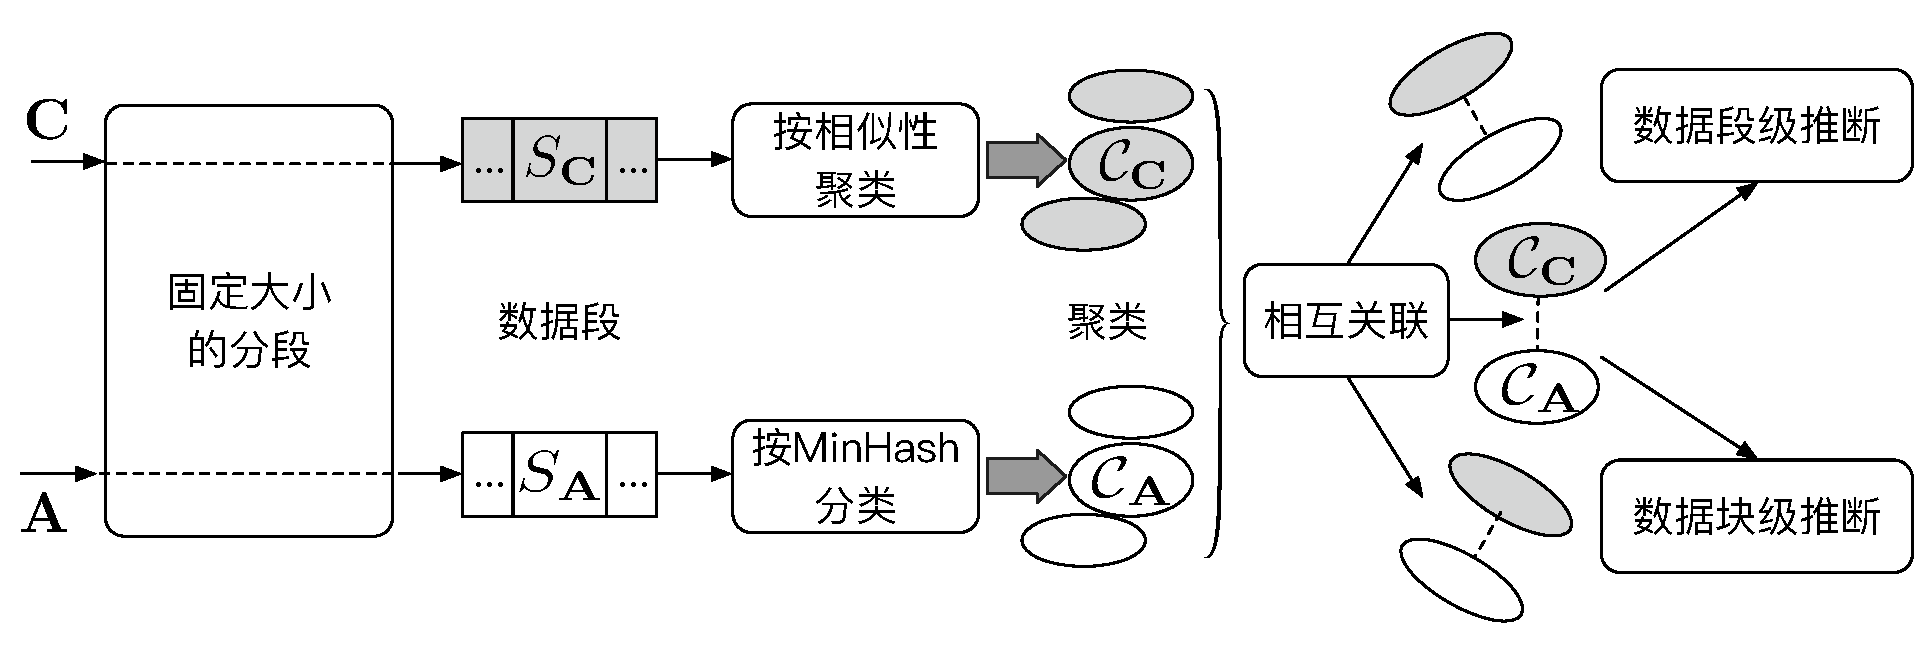
\includegraphics[width=14cm]{ClusteringAttack.eps}
    \caption{基于聚类的攻击方法的工作流程:用MinHash表示明文数据段的最小块散列} 
    \label{fig:基于聚类的攻击方法的工作流程}
\end{figure}

为了利用相似,本文首先在数据块概念的基础上引入数据段的概念。具体来说,将$\mathbf{C}$划分为为一些粗粒度的数据单元,成为密文数据段。密文数据段使用$S_\mathbf{C}$来表示,其中包含有$\mathbf{C}$中的多个相邻的密文数据块。在本课题中,应用了定长分段方法,以确保每个数据段具有相同分的大小(例如,默认大小为4MB)。同样的,对于攻击者所具有的辅助信息$\mathbf{A}$,也同样使用定长分段方法产生多个明文数据段,每个数据段由$S_\mathbf{A}$表示。

注意,一些可变大小的分段方案\citing{lillibridge2009sparse,qin2017design}在其内容与特定模式匹配的数据块之后设置分段边界,从而解决固定大小分段方案所面临的边界移位问题。但是,本文不能在攻击中使用这些可变大小的分段方案\citing{lillibridge2009sparse,qin2017design}。其原因是密文数据段中的数据块的原始内容受到对称加密的保护,攻击者无法确保密文和明文数据段的边界匹配采用的是相同的模式。该问题会导致密文和明文数据段不兼容,从而会降低基于聚类的攻击方法所推理的数据段级的数据量(请参阅本章后半部分)。
 
本方法通过类似的数据段来推理密文-明文对。给出$S_\mathbf{M}$是对应于密文数据段$S_\mathbf{C}$的明文数据段(即$S_\mathbf{M}$中的每个明文数据块对应于$S_\mathbf{C}$中的某些密文数据块,反之亦然)。根据Broder定理,如果一个明文数据段$S_\mathbf{M}$与辅助信息中的明文数据段$S_\mathbf{A}$具有相同的最小数据块哈希(称为$h$),则$S_\mathbf{M}$和$S_\mathbf{A}$可能拥有拥有大量相同的明文数据块。这意味着$S_\mathbf{C}$中的密文数据块很可能是从$S_\mathbf{A}$中的明文数据块映射得到的。换言之,攻击者首先按照最小数据块哈希对$\mathbf{A}$中的所有明文数据段进行分类,以此获得多个明文数据段集合(聚类的不同类别)。将每个明文数据段集合用$\mathcal{C}_\mathbf{A} = \{ S_\mathbf{A} \}$表示,对应于该集合中包含的所有明文数据段共有的唯一最小数据块哈希。同理,攻击者将密文数据段也进行上述分类操作,对于每个分类的集合用$\mathcal{C}_\mathbf{C} = \{ S_\mathbf{C} \}$表示)。然后,攻击者从对应于某一最小数据块哈希$h$的$\mathcal{C}_\mathbf{A}$中推理出$\mathcal{C}_\mathbf{C}$的原始明文数据。  

在本文中,定义任意两个密文数据段$S_\mathbf{C}$和$S_\mathbf{C}'$的聚类距离$d(S_\mathbf{C},S_\mathbf{C}')$为1减去相同密文的分数:

\begin{equation}
\label{eq:distence}
    d(S_\mathbf{C}, S_\mathbf{C}') = 1 - \frac{|S_\mathbf{C} \cap S_\mathbf{C}'|}{|S_\mathbf{C} \cup S_\mathbf{C}'|}.
\end{equation}

在推理过程中,相同的密文可能会在$S_\mathbf{C}$或$S_\mathbf{C}'$中重复出现,而$|S_\mathbf{C} \cap S_\mathbf{C}'|$和$|S_\mathbf{C} \cup S_\mathbf{C}'|$ 会分别返回其交集和并集中具有唯一性的密文数据块的数量。显然,$d(S_\mathbf{C}, S_\mathbf{C}')$越小,则说明$S_\mathbf{C}$和$S_\mathbf{C}'$更可能对应相同的最小数据块哈希。在本章中,采用凝聚法层次聚类(AHC)\citing{johnson1967hierarchical}方法来根据距离信息聚合相似的密文数据段。具体来说,攻击者从其拥有的每个密文数据段开始,将每个密文数据段视为一个单独的聚类类别,然后计算各个聚类之间的距离,将两个距离最近的(最相似的)聚类合并在一起,不断迭代这一过程直到任意两个聚类间的距离均大于给定最大距离参数$k$时停止迭代操作。
 
对于最终得到的每个密文聚类$\mathcal{C}_\mathbf{C}$,攻击者在考虑频率分布的前提下通过频率分析将其与一些明文聚类$\mathcal{C}_\mathbf{A}$相关联。该操作方法基于如下观察:相同的密文数据段(明文数据段)可以在相同或不同的密文数据段(明文数据段)中重复出现,并且相同的密文(明文)数据段也可以在相同的密文(明文)聚类中重复出现。同时,攻击者检查每个聚类中明文数据块或密文数据块的频率分布,并且认为相似的聚类(即,对应于相同的最小数据块哈希)中数据块的频率分布也是相似的。
 
本文按如下的顺序来设计频率分析攻击方案。首先,将所有可用的密文和明文聚类分别按它们包含的逻辑密文数据块和明文数据块的总数进行排序。然后,计算一个关联数组$\mathbf{F}$用于存储相应聚类中每个具有唯一性的密文数据块或明文数据块的频率。基于 $\mathbf{F}$,计算密文数据块$C$存在于密文聚类$\mathcal{C}_\mathbf{C}$中的概率$\Pr[C \in \mathcal{C}_\mathbf{C}]$,并进一步计算$\mathcal{C}_\mathbf{C}$的熵$e(\mathcal{C}_\mathbf{C})$:     

\begin{equation}
\begin{aligned}
\label{eq:Pr&eincluster}
    \Pr[C \in \mathcal{C}_\mathbf{C}] &= \frac{\mathbf{F}[\mathcal{C}_\mathbf{C}][C]}{\sum_{C' \in \mathcal{C}_\mathbf{C}} \mathbf{F}[\mathcal{C}_\mathbf{C}][C']} \\
    e(\mathcal{C}_\mathbf{C}) &= \sum_{C \in \mathcal{C}_\mathbf{C}} \log_2 \frac{1}{\Pr[C \in \mathcal{C}_\mathbf{C}]} 
\end{aligned}
\end{equation}

其中$\mathbf{F}[\mathcal{C}_\mathbf{C}][C]$存储了$\mathcal{C}_\mathbf{C}$中密文数据块$C$的频率。同理,计算出明文聚类$\mathcal{C}_\mathbf{A}$的熵$e(\mathcal{C}_\mathbf{A})$。与基于分布的频率分析攻击(参见\ref{sec:distribution-attack-description})类似,本文使用参数$(u, r, t)$来配置频率分析攻击方案。如果密文聚类$\mathcal{C}_\mathbf{C}$和明文聚类$\mathcal{C}_\mathbf{A}$满足如下三个条件则可说明两个聚类相似:   


\begin{itemize}
    \item  $\mathcal{C}_\mathbf{C}$的排名数值大小不大于$u$。
    \item  $\mathcal{C}_\mathbf{C}$和$\mathcal{C}_\mathbf{A}$的排名数值差距大小不大于$r$。  
    \item  $e(\mathcal{C}_\mathbf{C})$和$e(\mathcal{C}_\mathbf{A})$的差异是最小的,且不超过$t$.
\end{itemize}

然后,对于每个相似的聚类对$(\mathcal{C}_\mathbf{C}, \mathcal{C}_\mathbf{A})$,攻击者在两个级别分别进行明密文对的推理工作。

\begin{itemize}
    \item \textbf{数据段级推理}
    
    \par 如果$\mathcal{C}_\mathbf{C}$和$\mathcal{C}_\mathbf{A}$拥有相同数量的逻辑数据块(即密文数据块或明文数据块)以及相同的熵,则$\mathcal{C}_\mathbf{C}$与$\mathcal{C}_\mathbf{A}$完全映射的概率很高。在这种情况下,攻击者对粗粒度的数据段进行攻击。具体来说,攻击者首先在$\mathcal{C}_\mathbf{C}$中基于其密文的频率分布计算每个密文数据段$S_\mathbf{C}$的熵,并在$\mathcal{C}_\mathbf{A}$中基于其明文的频率分布计算每个明文数据段$S_\mathbf{A}$的熵。
         
         
    \par 如果$S_\mathbf{C}$和$S_\mathbf{A}$中逻辑数据块的总数和熵一致,则攻击者可以推理密文数据段$S_\mathbf{C}$是由命文数据段$S_\mathbf{A}$映射得到的。根据实验表明,基于聚类的频率分析攻击中大部分推理正确的内容来自于数据段级推理。同时,攻击者还可以利用额外的对抗性知识(例如,逻辑块顺序)来进一步恢复这些推理出的数据段中的每个数据块的明文。
         
    \item \textbf{数据块级推理}
    
    
    \par 如果$\mathcal{C}_\mathbf{C}$和$\mathcal{C}_\mathbf{A}$中具有的逻辑块数量或熵不同,攻击者对细粒度的数据块进行攻击。具体来说,攻击者分别对$\mathcal{C}_\mathbf{C}$和$\mathcal{C}_\mathbf{A}$中的具有唯一性的密文数据块和明文数据块按照出现频率进行排序,以此根据频率排名的顺序推理明文数据块-密文数据块对。            
     
    \par 然而,实验发现数据块级推理在本文给出的实验数据集中表现不佳。可能的原因是每个聚类包括大量逻辑数据块,这降低了频率分析的有效性。但即便如此,本文预计数据块级推理可以在实践中正确推理出更多的密文数据块-明文数据块对,当某些聚类中的逻辑数据块数量有限时效果会更佳。
 
\end{itemize}

\subsection{基于聚类的频率分析攻击方法总结}

总而言之,基于聚类的频率分析攻击利用相似性,在类似的聚类类别中使用频率分析攻击以推理密文数据块-明文数据块对。 除$u$,$r$和$t$外,它还由参数$k$配置,该参数指定了配对两个聚类类别的距离上限。

尽管可能受到固定大小数据段的边界偏移问题的影响,但本文认为基于聚类的频率分析攻击对VM磁盘映像的攻击效果是显著的。VM映像文件在创建时被分配了固定的大小,并且在其生存期内无法改变。在开始写入数据前,VM映像中的所有空间均由全零数据进行填充。在将数据存入映像的过程中,通过将需要用到的部分空间进行重写来完成数据存入过程。在章节\ref{sec:experiment-clustering}中,本文研究了针对VM磁盘映像的基于聚类的频率分析攻击的有效性。

\section{本章小结}

本章介绍了本文提出的第二种改进的频率分析方法:基于聚类的频率分析攻击方法。给出了该方法的相关背景知识、形式定义、方法描述以及最佳的适用场景。                  


